\chapter{Sketch It, Make It: Details}

The previous chapter gave an overview of SIMI's architecture. This
included an introduction of SIMI's recognition process.
(Section~\ref{sec:recognition-architecture}). This chapter gives
details on how each recognizer works. 

First, SIMI's corner finding and segmentation strategy is
described. This process is necessary to most recognition, and is what
produces geometric output like lines and arcs. Next, the three types
of recognizers are described: including Dynamic, Pen Up, and Delayed
recognizers. All sketch based interaction techniques are detailed in
these sections.

\section{Ink Parsing}
\label{sec:corner-finder}

Ink parsing is the process of identifying useful characteristics of
raw ink, such as the locations of corners, curvature at specific
points, and the likely identities of segments like lines or curves.

In the following sections, there are two different ways to measure
distance: Euclidean and Curvilinear (see
Figure~\ref{fig:distance-measures}). Euclidean distance is the
measurement most people are familiar with: this is how far apart two
points are on the 2D plane. Curvilinear distance follows the ink
stroke path. In the figure, points A and B are close together in the
Euclidean sense, but are farther apart in the Curvilinear sense. The
Euclidean and Curvilinear midpoints are also depicted in
Figure~\ref{fig:distance-measures}. 

\begin{SCfigure}%[t]
  \centering
  \caption[Euclidean vs. Curvilinear Distance]{Two ways to measure
    distance: Euclidean vs. Curvilinear. The Euclidean distance from A
    to B is direct ($length=18$). Curvilinear distance from A to B
    follows the path indicated ($length=86$). Each measurement
    approach has a related midpoint, indicated as smaller dots.}
  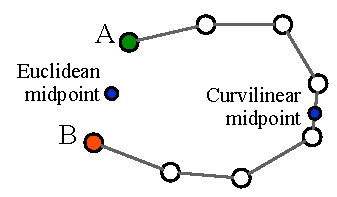
\includegraphics[width=3in]{img/distance-measures.pdf}
  \label{fig:distance-measures}
\end{SCfigure}


SIMI's ink parsing strategy is simpler than many other approches from
the SBIM literature. Others, like the strategies taken by
Sezgin~\cite{sezgin-early-processing} or Wolin~\cite{wolin-smr},
combine both \textit{time} and \textit{curvature} information when
corner finding. SIMI's approach relies only on curvature, but still
achieves good results.

When the user completes a stroke, the ink parser is invoked. First it
assigns a curvature value to each point. Next, a corner finder uses
this data to identify which (if any) points along the stroke are
corners. Last, the system analyzes the regions between corners to
determine the most likely segment type. The output of this process is
the set of segmets formed in the last step. I will detail each of
these steps now.

\subsection{Curvature}

\begin{figure}
  \centering
  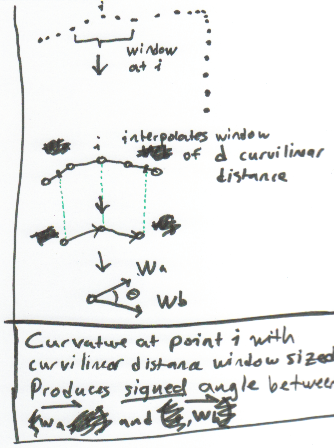
\includegraphics[width=2in]{img/curve-diagram.png}
  \caption[Curvature]{Illustration of how SIMI computes curvature about point $p_i$.}
  \label{fig:curvature-diagram}
\end{figure}


Figure~\ref{fig:curvature-diagram} illustrates how curvature is
calculated. A rough ink stroke has a series of points that are not
evenly spaced out. Sometimes, they may be very close together (for
example, when the user draws slowly). To determine the curvature at an
individual point, we must look at a nearby region called a
\textit{window}, rather than the immediate neighbors. Without this
window, the curvature would be unreliable when points are very close
together.

The window's size $w$ is determined by the current zoom factor. When
the zoom factor is 1 (meaning there is a 1:1 ratio between model and
screen coordinates), the window size is 20 (corresponding to 20
pixels). To calculate the window boundaries at point $p_i$, the corner
finder begins at $p_i$ and traverses the stroke backwards and forwards
by half the window size. It computes interpolated points $w_a$ and
$w_b$ that are exactly $w/2$ units along the stroke to $p_i$. It then
forms two vectors: $v_a$ from $w_a$ to $p_i$, and $v_b$ from $p_i$ to
$w_b$.

The signed curvature $\theta$ for $p_i$ is computed directly from
these two vectors. The magnitude is determined by their dot product;
the sign is determined by the cross product.

\begin{samepage}
\begin{equation}
  \theta_{unsigned} = \arccos \frac{v_a\cdot v_b}{|v_a| |v_b|}
\end{equation}

\begin{equation}
  \theta = \left\{ 
  \begin{array}{r l}
    \theta_{unsigned} & \quad \text{if } |v_a \times v_b| \geq 0\text{,}\\
    -\theta_{unsigned} & \quad \text{otherwise}\\
  \end{array} \right\}
\end{equation}
\begin{samepage}

It is tempting to use $\arctan$ to calculate curvature because it is a
simple calculation. However, this leads to discontinuities when the
vertical change is zero. The approach described above is valid for any
orientation.

\subsection{Isolate Corners}

Now that each point's curvature has been calculated, we can identify
corners. This is a two-step process illustrated
in~Figure~\ref{fig:corner-finding}. First, clusters of high curvature
are identified. To be a member of such a cluster, the absolute value
of a point's curvature must be greater than some threshold. In the
current version of SIMI this value is 45 degrees.

\begin{figure}
  \centering
  \begin{subfigure}[t]{0.4\textwidth}
    \centering
    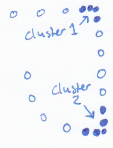
\includegraphics[width=1in]{img/corner-clusters.png}
    \caption{Clusters of high curvature.}
    \label{fig:corner-clusters}
  \end{subfigure}
  \hspace{1cm} % spacing, do what you need
  \begin{subfigure}[t]{0.4\textwidth}
    \centering
    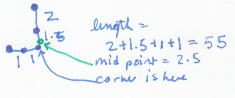
\includegraphics[width=2in]{img/corner-isolation.png}
    \caption{Corner point is closest to middle of cluster.}
    \label{fig:corner-isolation}
  \end{subfigure}
  \caption[Corner finding]{Corner finding involves clustering nearby
    points with high curvature, and choosing the point closest to the
    curvilinear middle of each cluster.}
  \label{fig:corner-finding}
\end{figure}


Once clusters have been computed, a corner is found for each. A
cluster's corner is simply the point closest to the curvilinear
middle. In other words, if the distance along stroke from the
beginning to the end of the cluster is 9, the corner is the point in
the cluster that is nearest to the interpolated point 4.5 units from
the cluster beginning. 

In addition to the corners discoved in this process, the stroke's
first and last points are also included as `corners'. This is for the
convenience of the next step where segments are identified.

\subsection{Identify Segment Types}

The last step in ink parsing is to identify segment
types. Table~\ref{tab:segment-types} in the previous chapter describes
the possible segment types. For each segment type there is a
corresponding segment finder. The segment finders for `open' types
(Line, Arc, Spline) operate on regions between corners. The remaining
segment finders are identified by examining the raw ink directly, and
do not use corner data.

Like semantic sketch recognizers, it is possible for multiple segment
finders to positivly identify ink. To mitigate this, segment finders
operate on a priority system. The priority is: Dot, Circle, Ellipse,
Blob, Line, Arc, and Spline. In other words, if the Dot finder
identifies a dot, there is no possibility of the associated ink being
identified as a Circle.

\subsubsection{Dot Finder}

The dot finder examines the entire ink stroke. If the entire stroke
was made in less than some threshold value (currently 180
milliseconds), it is always considered a dot. Otherwise, it continues
by computing the convex hull of all stroke points. Two properties of
the hull are used next: the area and the aspect ratio. If the ratio
defined by $ratio = area/aspect$ is less than 120, it is a dot. If
not, there is one final check to make. The stroke's point density is
computed. This is the number of points in the original ink stroke,
divided by the hull's area. If $ratio/(0.3 + density)$ is less than
120, it is a dot.

%% The thresholds used in this section (and many others) were determined
%% by trial and error. Some (such as point density) might need to be
%% changed dramatically if different hardware is used. For example, these
%% numbers were found using a default mouse driver, which reports only
%% integer positions. Ink strokes will be less dense than if a proper
%% tablet driver reports floating point locations.

\subsubsection{Circle and Ellipse Finder}

Circles, Ellipses, and (in the next part) Blobs are the three
\textit{closed} segment types. A segment is closed if the begining and
end points are close, relative to the overall length of the
stroke. More formally given start and end points $p_{start}$ and
$p_{end}$:

\begin{equation}
\begin{array}{rcl}
closeness &
= &
\dfrac{EuclidianDistance(p_{start}, p_{end})}{CurvilinearDistance(p_{start}, p_{end})} &
\\
closed &
= &
\left\{ 
  \begin{array}{r l}
    true & \quad \text{if } closeness \leq .1\text{,}\\
    false & \quad \text{otherwise}\\
  \end{array} \right\} \\
\end{array}
\end{equation}

Circles and Ellipses are identified with the same finder. If the input
stroke is closed, the input is fit to an ellipse. To avoid placing
restrictions on how users can draw, user may draw ellipses at
arbitrary angles. SIMI implements a least squares approach described
by Fitzgibbon \textit{et. al}~\cite{fitzgibbon-ellipse-fitting}. It is
an efficient algorithm whose complexity grows linearly with the size
of the input. The output of the ellipse fitting algorithm is a rotated
ellipse, defined by a centroid, a rotation, and major and minor axis
magnitudes.

An error value is calculated to determine how closely the raw input
matches the derived ellipse. This is done in a modified \textit{least
  squares} fashion that requires the calculating the minimum distance
between a point and the ellipse. Unfortunately this is an involved
process (for example, see ~\cite{eberly-point-to-ellipse}). SIMI
approximates the shortest distance between a point $p$ and an ellipse
by discretizing the ellipse boundary into a list of points $d$, and
computes the minimum distance between $p$ and $d$.

The error value measuring the closeness between raw input points $p_i,
i \in [0..n)$ and the discretized elliptical surface $D$ is given with
  the equation:

\begin{equation}
Elliptical\:Error = \frac{
\sqrt{
\sum min^2(p_i, D)
}
}{
n-2
}
\end{equation}

In order for the input to be considered a Circle or Ellipse, the total
error must be less than 1.0. This value was determined experimentally,
given a discretization of 60 points. To distinguish between a Circle
and an Ellipse, the fit ellipse's eccentricity used. Eccentricity
describes how flattned the ellipse is is defined in terms of its major
and minor radii:

\begin{equation}
Eccentricity = \sqrt{\dfrac{major^2-minor^2}{major^2}}
\end{equation}

If the eccentricity is less than 0.7, the input is a Circle; otherwise
it is an Ellipse.

\subsubsection{Blob Finder}

\subsubsection{Line Finder}

\subsubsection{Arc Finder}

\subsubsection{Spline Finder}

\section{Dynamic Recognizers}

\subsection{Erase}

What is it for? State obvious use quickly, and give detail on any
non-obvious uses.

Recognition process: What kind of data does it use? What is the
context-free recognition like? What context does it use?

What (if any) visual feedback is there?

What actions are taken if it is positively recognized and not
filtered?

Wrote this somewhere else: For example, the Erase gesture went through
a number of design iterations. Each version was only slightly better
than the last, and users were only able to successfully execute the
scribble gesture about half the time. When it failed, the scribble
would be interpreted as linework, which would then require users to
erase that. I then completely changed the erase gesture recognizer so
it would operate as the pen was down. When it found a scribble, a
colored 'X' appeared over the scribble to indicate that the user's
erasure will succeed. This lets users scribble until an X appears,
giving them confidence the system has understood. This reduced the
number of recognition errors substantially.

\subsection{Undo and Redo}

What is it for? State obvious use quickly, and give detail on any
non-obvious uses.

Recognition process: What kind of data does it use? What is the
context-free recognition like? What context does it use?

What (if any) visual feedback is there?

What actions are taken if it is positively recognized and not
filtered?

\subsection{Flow selection}

What is it for? State obvious use quickly, and give detail on any
non-obvious uses.

Recognition process: What kind of data does it use? What is the
context-free recognition like? What context does it use?

What (if any) visual feedback is there?

What actions are taken if it is positively recognized and not
filtered?

\section{Pen Up Recognizers}

\begin{itemize}
\item Remove hooks
\item Get structured ink related to unprocessed ink.
\item Add all new structured ink to the model
\item Apply post-hoc recognizers to new structured ink
\item Disambiguate any conflicting results using (a) context in the
  model and (b) preset rules like right-angle wins over same-length
  (filterRecognizedItems())
\item Apply remaining recognized items. This removes the related
  structured ink from the model.
\item Auto-latch remaining segments with each other and existing model
  segments.
\item Search for cutouts (don't call them stencils anymore)
\item Wake up constraint solver
\item Request state snapshot
\end{itemize}

\subsection{Latching}

What is it for? State obvious use quickly, and give detail on any
non-obvious uses.

Recognition process: What kind of data does it use? What is the
context-free recognition like? What context does it use?

What (if any) visual feedback is there?

What actions are taken if it is positively recognized and not
filtered?

Four kinds: automatic, endpoint, continuation, and t-junction.

\subsection{Pan and Zoom}

What is it for? State obvious use quickly, and give detail on any
non-obvious uses.

Recognition process: What kind of data does it use? What is the
context-free recognition like? What context does it use?

What (if any) visual feedback is there?

What actions are taken if it is positively recognized and not
filtered?

\subsection{Select point}

What is it for? State obvious use quickly, and give detail on any
non-obvious uses.

Recognition process: What kind of data does it use? What is the
context-free recognition like? What context does it use?

What (if any) visual feedback is there?

What actions are taken if it is positively recognized and not
filtered?

\section{Delayed Recognizers}

\subsection{Same length}

What is it for? State obvious use quickly, and give detail on any
non-obvious uses.

Recognition process: What kind of data does it use? What is the
context-free recognition like? What context does it use?

What (if any) visual feedback is there?

What actions are taken if it is positively recognized and not
filtered?

\subsection{Specific length}

What is it for? State obvious use quickly, and give detail on any
non-obvious uses.

Recognition process: What kind of data does it use? What is the
context-free recognition like? What context does it use?

What (if any) visual feedback is there?

What actions are taken if it is positively recognized and not
filtered?

\subsection{Right angle}

What is it for? State obvious use quickly, and give detail on any
non-obvious uses.

Recognition process: What kind of data does it use? What is the
context-free recognition like? What context does it use?

What (if any) visual feedback is there?

What actions are taken if it is positively recognized and not
filtered?

\subsection{Same angle}

What is it for? State obvious use quickly, and give detail on any
non-obvious uses.

Recognition process: What kind of data does it use? What is the
context-free recognition like? What context does it use?

What (if any) visual feedback is there?

What actions are taken if it is positively recognized and not
filtered?
